\chapter{General discussion, future work and conclusions}
\label{ch:conc}
\acresetall

%Antarctic lakes are exceptional ecosystems that contain microbial life adapted to extreme polar conditions and the local lake geochemistry.
Metagenomics has proven to be an effective way to map the diversity of Antarctic lake ecosystems and provide hints of how they work.
In combination with metaproteomics and abiotic parameters, in-depth descriptions were achieved of the ecosystem functions of Ace Lake and Organic Lake.
The most noteworthy contribution of these studies has been to describe taxa and microbial processes previously unknown in these lakes, and from these descriptions, generate testable hypotheses of population and ecosystem level function.
\section{Possibile future work on Organic Lake}
%The work described in this thesis is part of a program that has pioneering the use of shotgun metagenomics and metaproteomics in Antarctic lakes \cite{Ng2010a, Lauro2011, Yau2011} and the Southern Ocean \cite{Wilkins2012b, Grzymski2012, Williams2012a, Williams2012b}.
To establish a picture of the biotic composition and function of Antarctic lake communities, an observation-driven approach was utilised that allowed for completely new discoveries about these systems to be made.
Bioinformatic pipelines and theoretical models to do this have now been established.
These can be applied to future, similarly observation-based studies of Ace and Organic Lakes to define how they change over time and test our existing models of how the lakes function.
It is also clear that a systems level understanding of the lakes is bolstered by having well-characterised isolates related to members in the community.
Guided by the studies from this thesis, isolation and characterisation of key members of the community, such as \emph{Pyramimonas} spp., \ac{OLPV}, \ac{OLV}, \emph{Marinobacter} spp. and \emph{Roseovarius} spp. from Organic Lake, could be attempted in the future.
Other complementary techniques, such as single-cell and single-virus genomics and \ac{SIP}, hold promise for learning about specific populations in the community.
Some experiments that could be used to test specific hypotheses generated by the study of Organic Lake are discussed below, along with their expected outcomes and implications.

\subsection{Organic Lake community dynamics}
To establish a complete understanding of Organic Lake requires descriptions of the microbial community over different time scales.
Certain bacterial taxa have been observed to peak in abundance in Organic Lake during summer indicating seasonal fluctuations exist \cite{James1994}.
The Organic Lake community profiles from the summer of 2006 and 2008 varied substantially (chapters \ref{ch:olv} and \ref{ch:org}) identifying further community members that change with time.
However, the rates of change and degree of variance for these populations are unknown.
%It is also possible the Organic Lake community varies between years, for example with variations in climatic conditions.
Currently, a baseline of the microbial community diversity over an annual cycle has not been established and is the next step required for improved modelling of the Organic Lake ecosystem.

%This is a necessary benchmark to determine if inter-seasonal variations exist.
Metagenomic and functional data obtained over the course of a year can determine how the microbial community responds to the large seasonal changes in temperature, light and ice-cover.
Winter samples in particular can establish how the community persists when the lack of light is expected to curtail photosynthetic production.
Paired metagenomic and metaproteomic analyses of the coastal Southern Ocean from winter and summer found winter samples were dominated by active chemolithoautotrophs including sulphur-oxidising \emph{Gammaproteobacteria} and ammonia oxidising \emph{Crenarcheaota} \cite{Grzymski2012, Williams2012b}.
If the Organic Lake ecosystem reflects that of the coastal Southern Ocean, the small population of chemolithoautotrophic sulphur-oxidising \emph{Proteobacteria} found to be present (chapter \ref{ch:org}) are expected to become dominant in the winter.
%Succession of the summer bacterial population by \emph{Crenarchaeota} is not expected to occur as no signatures for \emph{Crenarchaeota} or ammonia oxidation were present in Organic Lake.
Metagenomic analysis indicated recycling of reduced nitrogen compounds predominates in Organic Lake (chapter \ref{ch:org}).
If this model of nitrogen cycle holds true over the year, we can expect ammonia oxidising microorganisms will not play a part in the community as they do in other similar environments \cite{Voytek1999, Grzymski2012, Williams2012b}.
%Another possibility is that some bacterial populations become dormant over the winter, as seems to occur in Artic sea ice communities \cite{Collins2010}.

Photosynthetic nanoflagellates detected in Organic Lake, such as \emph{Pyramimonas}, are capable of mixotrophy \cite{Bell2003} and likely persist over the winter by switching to heterotrophy \cite{Laybourn-Parry2005}.
Strategies that might also be employed by other photosynthetic algae include utlising starch reserves or encysting \cite{Laybourn-Parry2002}.
In Lake Bonney, trends between \acs{RuBisCO} expression and irradiance levels differed with \acs{RuBisCO} type and depth suggesting adaptations to the polar night varies between species \cite{Kong2012a}.
Phototrophic eucaryotes in Organic Lake likely have similarly diverse strategies to persist during prolonged darkness.
Combined metagenomic and metaproteomic analysis can determine which phototrophic eucaryotes are found during the winter and indicate what metabolic processes they employ in the absence of light.

%Ideally, metagenomic analyses performed over a  complete annual cycle would establish a census of the community, link variations in composition to environmental conditions and establish a benchmark of annual variability in the community.
Some members of the Organic Lake population appear to be persistent over long time scales.
For example, \emph{Dunaliella} \cite{Franzmann1987b}, choanoflagellates \cite{vandenHoff1986}, \emph{Marinobacter}, \emph{Psychroflexus} \emph{Roseovarius} and \emph{Halomonas} \cite{Bowman2000a} have been recorded in Organic Lake previously and were detected again in studies from this thesis (chapters \ref{ch:olv} and \ref{ch:org}).
How they vary throughout the year and between years is unclear.
Organic Lake has been shown to be physically variable over a decadal time scale with changes in water level of $\sim$1 m leading to large changes in the water column structure \cite{Gibson1995, Gibson1996}.
Notably, the pycnocline in Organic Lake occurred at 5.7 m in 2008; much lower than 3.5 m where it first reported in 1978 \cite{Franzmann1987b}.
If the lake completely mixes, this would challenge the oxygen-senstitive microbes and processes occurring in the deep zone.
In West Antarctic lakes, physical changes have been correlated with large and rapid ecological responses \cite{Quayle2002}.
Substantial differences were observed in \emph{cbbM} gene copy number and vertical distribution between three field seasons in Lake Bonney \cite{Kong2012b} indicating sensitivity to environmental factors also applies to permanently ice-covered lake ecosystems and is a general property of Antarctic lakes.
However, the amount of seasonal variability needs to be established in Organic Lake for differences over longer time scales to be determined.

%Long-term sampling of Southern Ocean coastal surface waters suggests the community has a reproducible annual cycle \cite{Murray2007}.
Sampling over the course of a summer season would be particularly valuable as these samples can be compared to the available summer datasets to give a better indication of the degree of variability between summer seasons.
There was a change in the viral composition and abundance between November and December 2008 samples when the lake began to thaw (chapter \ref{ch:olv}).
Similarly, there were differences in the eucaryotic community when the lake was completely thawed in 2006 (chapter \ref{ch:olv}) and the profile in November 2008 when the lake was ice-covered (chapter \ref{ch:org}).
%This suggests shifts in the microbial community is related to ice-cover melt and/or increased solar irradiance. 
%Specifically, \emph{Dunaliella}, \emph{Dictyochophyceae}, \emph{Euplotes}, \emph{Dinophyceae} and \emph{Bacillariophyta} were present in both samples, whereas \emph{Pyramimonas}, \emph{Pelagophyceae}, \emph{Pirsonia} and \emph{Caecitellus} was only detected in the December 2006 samples and fungi and \emph{Choanoflagellida} were only in the November 2008 profile (chapter \ref{ch:org}).
It is unclear whether the variation between the summer samples is due to differences in ice-cover/light, sampling locations  (2006 and December 2008 samples were littoral, while November 2008 was over the deepest point of the lake) or other environmental factors.
Metagenomic sequencing of a summer time course would provide a high resolution view of changes in the microbial community over the season that can be related to environmental conditions.
This time course can be compared back to the summer 2006 and 2008 samples indicating if the differences that have been observed fall within normal range of variability over the summer season and also help interpret what factors were driving those variations.

Metagenomic sequencing of samples from a summer time course can also validate the \ac{OLV}--\ac{OLPV}--host model formulated in chapter \ref{ch:olv}.
Genomic analysis indicated \ac{OLV} is a new member of the virophage virus family, which uses \ac{OLPV} as a `helper' virus to complete its replication cycle but impairs its helper's infectivity in the process.
The likely host of \ac{OLV} and \ac{OLPV} was determined to be the unicellular alga, \emph{Pyramimonas}.
The inferred interaction of the \ac{OLV}, \ac{OLPV} and host was used to generate a Lotka-Volterra model of their population dynamics that showed if \ac{OLV} acts as a `predator of a predator', this would lead to increased frequency of population cycles.
Observations of changes in \ac{OLV}, \ac{OLPV} and \emph{Pyramimonas} abundances over a summer time course can establish if a relation exists between them.
An observable trend between these populations would lend further support to the claim that \ac{OLV}--\ac{OLPV} and \emph{Pyramimonas} are a virophage--virus--host system.
In the model, the density of each population oscillates in a phase-shifted manner in the sequence: prey, predator and predator of predator.
Observed population changes can determine if the data fits the model, suggest if additional modifications to the existing model need be made or if alternative models would better fit the data.
If the dynamics fit the model, observed population densities can be used to derive the parameters that govern their interaction.

\subsection{\acs{OLV} physiology and ecology}
Since the discovery of the \ac{OLV}, two other members of the virophage family have been reported that have afforded a new perspective on \ac{OLV}.
The first of these is the Mavirus (for Maverick virus) so named for its evolutionary relationship with the Maverick/Politon class of eucaryotic transposons \cite{Fischer2011a}.
Like Sputnik, Mavirus has an absolute requirement for a helper virus, \ac{CroV}, to replicate and is deleterious to its helper \cite{Fischer2011a}.
The other virophage reported was called Sputnik 2 (its genome is almost identical to Sputnik), but unlike Sputnik, it was found both as a separate genome and integrated in its helper lentille virus \cite{Desnues2012}.
These two virophage systems in culture are associated with heterophic protists making \ac{OLV} the only genomic sequence currently available for virophage affecting cosmopolitan phytoplankton species.
Therefore isolating \ac{OLV}, acquiring genomes of \ac{OLV} relatives in Antarctic lakes and determining fundamental properties of \ac{OLV} physiology and dynamics would contribute immensely to our understanding of the evolution and diversity of virophages in general and is highly relevant to other aquatic systems.

The evidence that Mavirus has the same `virophage' phenotype as Sputnik strengthens the inference that \ac{OLV} does as well.
This is in part because Mavirus and \ac{CroV} and quite divergent from Sputnik and mimivirus respectively, yet retain the same traits \cite{Fischer2010, Fischer2011a}, suggesting a common feature of the whole lineage.
Moreover, as both mimivirus and \ac{CroV} encode much of their transcriptional machinery, they do not localise to the nucleus during infection but generate the viral factory in the cytoplasm of their host \cite{LaScola2008, Fischer2010}.
Sputnik and Mavirus appear to replicate in the giant virus factory making use of helper virus' replication and transcription systems, not the host cell's \cite{LaScola2008, Claverie2009, Fischer2011a}.
In this way, the replicative strategy of the mimivirus lineage makes them vulnerable to virophages parasitising necessary resources during replication, which is a likely cause of reduced helper virus production \cite{Claverie2009, Fischer2011a, Fischer2011b}.
As \ac{OLPV} encodes all \textsc{RNA} polymerase subunits (see GenBank accession HQ704802), this is evidence that it replicates solely in the cytoplasm, thereby making it susceptible to a virophage.
A larger census of virophage and helper viruses would be able to show if virophages only associate with members of the \ac{NCLDV} clade that replicate in the cytoplasm.
Ultimately, definitive confirmation of a detrimental effect on the helper during \ac{OLV} co-infection is likely only possible by observing infection in culture.

Although Sputnik and Mavirus have similar effects on their helper viruses, their infection strategies appear different raising interesting considerations for \ac{OLV}.
%All three genomes have share homologues of the Sputnik V20 \ac{MCP}, V3 FstK-HerA DNA packaging ATPase and V9 putative cysteine protease but otherwise are quite divergent.
%Sputnik and Mavirus additionally share a the V13 primase/superfamily 3 helicase and the V14 Zn-ribbon domain containing protein.
%While Sputnik and \ac{OLV} share the V18/19 minor virion protein, V1 primase-polymerase containing protein and V21 hypothetical protein.
Mavirus can be independently phagocytosed by \emph{Cafeteria roenbergensis} in the absence of \ac{CroV} -- perhaps serving as a defence for the host in the case of \ac{CroV} infection \cite{Fischer2011a}.
In support of this, Mavirus possesses a retroviral-family integrase that is theorised to have been separately acquired as a way to stabilise the relationship between the ancestral Mavirus and its cellular host \cite{Fischer2011a} although as yet, Mavirus has not been reported to be integrated in \emph{Cafeteria roenbergensis}.
In contrast, Sputnik seems to associate directly with the fibrils that coat the mimivirus virion, not the host \emph{Acanthamoeba} cell \cite{Boyer2011}.
These two modes of infection, that is, a virophage-bearing host being infected by a giant virus \emph{vs}. a host being infected by a virophage-bearing giant virus, produces different selection pressures that would lead to distinct effects on the population dynamics in the environment.
Detection of complete \ac{OLV} genomes in the 0.8--0.1 \textmu{}m size fraction indicates it was captured in association with larger particles but does not distinguish how it is transmitted.

Determination of the mode of infection for \ac{OLV} would improve predictive modelling of \ac{OLV} driven impacts on algal blooms.
This could be achieved by observation of \ac{OLV}-\ac{OLPV} infections in culture.
However, recently developed methods for flow cytometric sorting to obtain \acp{SAG} or \acp{SVG} \cite{Martinez-Martinez2011, Allen2011} could be applied to Organic Lake water samples to study the mode of \ac{OLV}, \ac{OLPV} and host interaction.
For example, a sample population of single host algal cells could be fluorescence sorted and screened for the presence of \ac{OLPV} and \ac{OLV}.
At the same time, a sample population of single \ac{OLPV} particles could be sorted and screened for the presence of \ac{OLV}.
This could reveal if \ac{OLV} is able to associate with the host independently of \ac{OLPV} or \emph{vice versa}.
Examination of the infected algal cells could also establish fundmental properties of the algae and virus populations such as proportions of infected cells and proportions of \ac{OLPV} infections that include an \ac{OLV}.
As these methods are quite new, an experiment of this kind would require optimisation to successfully capture an adequate sample of infected cells and target giant viruses.
However, just obtaining \acp{SVG} would provide invaluable information on virus diversity and genetic content making it worthwhile pursuing as a complement to metagenomic sequencing.

A final consideration for \ac{OLV} and \ac{OLPV} dynamics is suggested by the discovery that Sputnik 2 can integrate into its helper lentille virus \cite{Desnues2012}.
Integration of Sputnik 2 is localised to a 352 bp region corresponding to the Sputnik V6 gene that encodes a collagen-like repeat-containing protein shared by Sputnik 2, lentille virus and mamavirus  \cite{Desnues2012}. 
\ac{OLV} and \ac{OLPV} share a homologous collagen-like repeat-containing protein that may similarly function as a site of integration.
As yet, the conditions and mechanism by which Sputnik 2 integrates is unknown.
Screening of metagenomic assemblies, \acp{SVG} or isolated \ac{OLPV} genomes for integrated virophages can determine if this occurs in the environment.
Integration of \ac{OLV} and \ac{OLPV} could have interesting evolutionary functions.
One possibility is that integration of virophages may function analogously to lysogeny in bacteriophages if provirophages are inactive.
In this scenario, virophages would integrate into their helper virus when helper virus densities are low to avoid driving their helpers to extinction.
On the other hand, if integration does not entail dormancy of the virophage, it could function as a means to ensure transmission.
In either case, evidence of integration can be found in future genomic studies of Organic Lake.

\subsection{Organic lake biogeochemistry}
The models of carbon, nitrogen and sulphur cycling in Organic Lake were constructed based on the presence and abundance of known marker genes  along with data of the lake's chemical properties (chapter \ref{ch:org}).
As yet, metaproteomic analyses from the same samples have not been performed, but this would help corroborate the inferred pathways are active. 
Other inferrences of Organic Lake biogeochemical function can be specifically tested on organisms in culture, tested by measuring rates of reaction \emph{in situ} or supported with additional molecular and chemical analyses.

For the carbon cycle, it was hypothesized that \ac{AAnP} and rhodopsin mediated photoheterotrophy can conserve carbon for use in biosynthesis  reducing overall carbon loss (chapter \ref{ch:org}).
The conditions under which \ac{AAnP} is active can be tested on related organisms in culture, for example \emph{Roseovarius tolerans} from Ekho Lake in the Vestfold Hills. 
It is already known for \emph{R. tolerans} constant dim light suppresses \ac{BchlA} production while darkness stimulates it \cite{Labrenz1999}.
\emph{R.tolerans}, or related isolates, can be grown under a larger range of conditions to determine when \ac{AAnP} becomes an active process.
This might include further varying light intensity and cycle duration; varying organic carbon concentration and oxygen concentrations.
To determine the contribution of light to growth, the difference in growth when \ac{AAnP} is active and when it is not can be compared.
Characterising \ac{AAnP} in a model isolate from a similar Antarctic lake can inform an understanding of how it functions in Organic Lake.
However, to gain an understanding of when \ac{AAnP} is active \emph{in situ}, levels of \ac{BchlA} at different points in the year can be measured to see it correlates with seasonal changes.
In the case of the influence of rhodopsin-mediated phototrophy on the Organic Lake system, the function of rhodopsins first needs to be characterised in the diverse organisms in which they are found to confirm they are indeed used in photoheterotrophic growth.
In marine \emph{Flavobacteria}, there is already evidence that light stimulates growth through the action of rhodopsins \cite{Gomez-Consarnau2007}.
The same experimental design used to establish this can be applied to \emph{Psychroflexus gondwanensis} isolated from Organic Lake, \emph{Marinobacter} sp. ELB17 and \emph{Octadecabacter antarcticus}, which are relatives of species found in Organic Lake.

In the model of the nitrogen cycle, nitrogen fixation was inferred to be negligible due to the high concentrations of ammonia while denitrification was assumed to be limited by low levels of oxidised nitrogen compounds and lack of potential for nitrification to regenerate them (chapter \ref{ch:org}).
In these cases where rates of reaction were inferred to be slow although genetic potential for them exists, the reaction rates can be directly measured.
Nitrogen fixation and denitrification rates can be measured from Organic Lake water samples by incubation with $^{15}$N labelled substrates or acetylene block assays.
Similarly, it was inferred that carbon fixation rates from photosynthetic algae and chemolithoautotrophic bacteria were lower than respiration and fermentation based on genetic potential (chapter \ref{ch:org}).
As mentioned previously, populations of chemolithoautotrophs may increase in the winter, potentially becoming signficant source of primary production.
Another consideration for the carbon budget is how sustained levels of chemolithoautotrophy throughout the year compares to the short burst of photosynthetic production over the summer.
Continuous rates of chemolithoautotrophy appears to occur in Lake Bonney in McMurdo Dry Valleys as their expression of \acs{RuBisCO} remained constant over the polar night transition \cite{Kong2012b}.
Measuring rates of primary production by $^{14}$C incorporation and respiration rates at different points in the season can acertain if there truly is a shortfall in the carbon budget in Organic Lake, estimate how large it is and pinpoint if the main source of primary production is from photo- or chemoautotrophy.

Both the carbon and nitrogen cycles were also constructed with the assumption that inputs are also negligible.
For instance, denitrification rates would be limited by low fixation coupled with low rates of nitrification.
Nonetheless, it is possible that sufficient nitrate inputs occur that would sustain denitrification thereby by-passing the need for endogenous nitrification.
Monitoring for presence of melt streams that might feed into Organic Lake and determining their chemical profiles can gauge the contribution of allochtonous carbon and nitrogen to Organic Lake.

The unusually high concentrations of \ac{DMS} in the bottom waters of Organic Lake were inferred to originate from bacterial lysis of \ac{DMSP} (chapter \ref{ch:org}).
As \ac{DMSP} lyases have only been discovered fairly recently \cite{Todd2007, Curson2008}, they have only been characterised from a few isolates \cite{Todd2007, Curson2008, Curson2010, Todd2010, Curson2012}.
Confirmation that the homologues found in Organic Lake are indeed functional can be achieved by cloning into the expression vector system established by \citet{Todd2007} and assaying for \ac{DMSP} lyase activity.
This would also provide valuable insight into the \ac{DMSP} lyases that are most relevant to cold and hypersaline environments.

Although it was inferred that \ac{DMSP} lysis was the main source of \ac{DMS} in the bottom zone of Organic Lake, production of \ac{DMS} other by anaerobic pathways are also possible.
Furthermore, \ac{DMS} was inferred to accumulate due to slow rates breakdown in the bottom zone.
Incubating Organic Lake water samples with radio-labelled \ac{DMSP} and tracking production of volatile \ac{DMS} would confirm the lysis pathway is an active process and determine the rates of reaction.
Performing this assay on water from different depths could determine if concentration of \ac{DMS} is high in the bottom zone because it is being produced there at a higher rate.
A similar assay can be performed using labelled \ac{DMS} to show if \ac{DMS} can be broken down and if this differs with depth.
If the proposed model for sulphur cycling based on marker gene frequencies is correct, \ac{DMS} breakdown in the bottom samples should be slow or not occur.
While this experiment will not exclude the possibility that \ac{DMS} is produced by an alternative pathway, knowing the rates of \ac{DMSP} lysis and \ac{DMS} breakdown and the \ac{DMS} concentration in a sample can indicate the existence other sources of \ac{DMS} production.

Most of the Organic lake \ac{DMSP} lyase genes could be linked to a taxonomic group except the most abundant type, OL-dddD, which had indication of both \emph{Alpha}- or \emph{Gammaproteobacteria} origins (chapter \ref{ch:org}).
Identifying the organisms involved in \ac{DMSP} lysis can be achieved with \ac{SIP}.
This would involve incubation of $^{13}$C-labelled \ac{DMSP} in Organic Lake water samples followed by sequencing of the labelled DNA.
Sequencing of the \ac{SSU} genes would determine which specific taxonomic groups were the main contributors to \ac{DMSP} lysis and screening for \ac{DMSP} lyase genes would identify which \ac{DMSP} lyase is involved.
Performing this experiment at different depths of the water column could determine if the same organisms are responsible for \ac{DMSP} lysis at different depths.
No marker genes yet exist for \ac{DMS} oxidation although it can be readily utilised as a growth substrate by diverse microorganisms \cite{Johnston2008}.
The same experiment can be performed using $^{13}$C-labelled \ac{DMS} to determine the taxa involved in breaking it down in different depths of the lake.
In conjunction with metagenomic sequencing, or flow sorting and \acp{SAG} of \ac{DMS}/\ac{DMSP}-degraders, the biochemical pathways involved in \ac{DMS} breakdown can then be reconstructed giving a more complete understanding of Organic Lake sulphur biogeochemistry.

\section{Perspectives on `-omics' approaches }
It was not so long ago that what could be called the second molecular revolution in microbial ecology began in earnest with the first shotgun metagenomic sequencing of a marine virome \cite{Breitbart2002}.
That metagenome, sequenced with Sanger sequencing technology, was a modest 1.28 Mbp \cite{Breitbart2002}.
The first shotgun sequenced metagenomes of cellular life from the Sargasso Sea \cite{Venter2004} and the Iron Mountain acid mine drainage \cite{Tyson2004} added 1 Gbp and 76 Mbp respectively to the public databanks.
Although this level of sequencing effort is now relatively small, it was enough to uncover hundreds to thousands of viral types of which 65\% bore no similarity to any known sequence \cite{Breitbart2002} and expand the breadth of known protein families including 782 previously unknown rhodopsin-like sequences \cite{Venter2004}.  
These studies were also revolutionary because they pioneered different ways of using shot-gun sequencing to look into the microbial world.
Where metagenomics applied to the higher diversity Sargasso Sea opened up a broad swathe of species and functional diversity \cite{Venter2004}, environmental sequencing applied to the lower complexity acid mine community enabled strain level differences of a few organisms to be resolved \cite{Tyson2004}.

\subsection{Next generation sequencing technologies}
Since the availability of high-throughput \ac{NGS} technologies, the volume of metagenomic data has increased exponentially.
%Currently, the Genomes Online Database (\url{http://www.genomesonline.org}) lists 2,350 metagenomic samples from 369 separate projects.
To put it in perspective, a single sample from the Antarctic lake datasets described in this thesis sequenced by the Roche GS-FLX titanium sequencer is 140 Mbp, while a recent study using Applied Biosystems SOLiD sequencing of a marine sample \cite{Iverson2012} analysed 55,000 Mbp -- close to 400 times the amount of data.
This illustrates how sequencing technology is advancing so rapidly that each new study has to develop new ways of looking into the microbial milieu captured in the particular sample.

Current \ac{NGS} sequencing platforms are shown in \tabreft{tab:seq_tech} comparing sequence length, throughput and error rates.
Clearly, there are trade-offs between each type with higher read depth technologies offering shorter read lengths. 
Application of sequencing technologies that offer greater read depths in future Antarctic lake studies can enable insight into the rare members of the community.
For example, a recent study compared \acs{SSU} community profiles over a six year time course with a single sample deep-sequenced with the Illumina GAIIx platform \cite{Caporaso2012}.
Members of the community that appeared to become seasonally absent in the shallow sequenced community profiles were actually present in low abundances in the deep-sequenced sample \cite{Caporaso2012}.
The ability to look into deeper into diversity of the Antarctic lake communities can discern if a similar persistent `seed bank' population exists in the lakes, if succession of populations occurs or external seeding.
These three different possibilities have different implications for predicting responses to change in environmental conditions in the lakes.
It also illustrates how \ac{NGS} can be used for hypothesis-driven analysis and not just as a tool for discovery.
%The long read length offered by single-molecular sequencing (Pacific Biosciences) is off-set by a high error-rate and has not as yet been applied to metagenomics.
\begin{table}
\footnotesize
\caption[Comparison of next generation \textsc{DNA} sequencing platforms]{Comparison of next generation \textsc{DNA} sequencing platforms from \citet{Scholz2012}. Indel, insertion-deletion; Sub, substitution; MP, mate pair; PE, paired end.
}
\label{tab:seq_tech}
\smallskip
\begin{tabularx}{\textwidth}{p{3cm}p{2.5cm}XXp{1.5cm}p{1.2cm}}
\toprule
\textbf{Platform} & \textbf{Run time (h)} & \textbf{Read length (bp)} & \textbf{Mbp/run} & \textbf{Error type} & \textbf{Error rate (\%)} \\
\midrule
\emph{Roche}             &        &                   &            &              &   \\
454 FLX$+$               & 18--20 & 700               & 900        & Indel        & 1 \\
454 FLX$+$ Titanium      &  10    & 400               & 500        & Indel        & 1 \\
454 GS                   &  10    & 400               & 50         & Indel        & 1 \\
\emph{Illumina}          &        &                   &            &              &  \\
GAIIx                    & 14     & 2 $\times$ 150    & 96,000     & Sub          & $>$0.1 \\
HiSeq 2000               & 8      & 2 $\times$ 100    & 400,000    & Sub          & $>$0.1 \\
HiSeq 2000 V3            & 10     & 2 $\times$ 150    & $<$600,000 & Sub          & $>$0.1 \\
MiSeq                    & 1      & 2 $\times$ 150    & 1,000      & Sub          & $>$0.1 \\
\emph{Life Technologies} &  &  &  &  &  \\
SOLiD 4                  & 12     & 50 $\times$ 35    & 71,000     & AT bias     & $>$0.06 \\
SOLiD 4                  & 12     & 75 $\times$ 35 PE & 155,000    & AT bias     & $>$0.01 \\
                         &        & 60 $\times$ 60 MP &            &             &  \\
\emph{Ion Torrent}       &        &                   &            &             &  \\
PGM 314 Chip             & 3      & 100               & 10         &  Indel      & 1 \\
PGM 316 Chip             & 3      & 100$+$            & 100        &  Indel      & 1 \\
PGM 318 Chip             & 3      & 200               & 1,000      &  Indel      & 1 \\
\emph{Pacific biosciences} &  &  &  &  &  \\
RS                       & 14/8 Smart Cells & 1,500 & 45/smart cell &  Insertions & 15 \\
\bottomrule
\end{tabularx}
\end{table}


\subsection{Emerging bioinformatic bottlenecks}
With the higher throughput and the falling costs of sequencing, genomic projects are now experiencing `bioinfomatic bottlenecks' where computational analysis has become a significant challenge (reviewed by \citet{Scholz2012}).
This is because availability of computational resources and scaling-up of algorithms to accomodate more data or computing clusters is not occurring as quickly as the accumulation of sequence data.
Metagenomic sequencing projects typically entail computationally intensive \acs{BLAST}-like comparisons before biological interpretations can be made.
Local cluster computing, like that used in this thesis, has been a standard way to process metagenomic datasets.
However, the annual cost of acquiring, running and administering a standard rack mount server has been estimated to be \$2,160--\$5,160 US per node \cite{Wilkening2009}.
Acquiring and maintaining the necessary computational resources to process large datasets can in some cases work out to be more expensive than the cost of sequencing itself.
Moreover, the time to acquire sequence data is much shorter than the time needed to analyse it.
For example, analysis of metagenomic data produced by Illumina technology using a standard pipeline was calculated to take decades on a single processor or weeks to months on 1,000 \acs{CPU}s \cite{Evanko2009}.
Without increases in compute resources, the time taken to process massive \ac{NGS} datasets will become prohibitively slow and is an important consideration for future metagenomic projects.

\subsection{Prospects for closing the bioinformatic gap}
Ultimately, for computational analysis to catch up with advances in sequencing technology more efficient processing, faster processors and faster algorithms are required.
Ways to surpass the bioinformatic bottleneck are being developed and, if theses advances are paired with careful experimental and analytical design, will enable computational challenges to be managed.

\subsubsection{Webserver analyses}
A shortage in computational resources can be addressed to some extent by the use of webserver pipelines specialised in metagenomic processing.
These include \acs{MG-RAST} \cite{Meyer2008}, \acs{CAMERA} \cite{Sun2011}, \acs{IMG/M} \cite{Markowitz2008, Markowitz2012}, EBI Metagenomics \cite{Hunter2012}, as well as \textsc{Metavir} \cite{Roux2011} and \acs{VIROME} \cite{Wommack2012} for viral metagenomes.
These webservers take on the burden of maintaining necessary programs, storage of sequence databases and provide computational power.
Each have unique features that may be more desirable for particular sample types, analyses or user preferences.
%One example of this is the different functional analyses offered by EBI Metagenomics and \ac{MG-RAST}, which implement InterPro and SEED subsystems respectively.
%In this thesis, use of \ac{CAMERA} was convenient for \acs{BLAST} searches of \ac{OLV} against all other metagenomes (chapter \ref{ch:olv}) as it saved from having to download large metagenomic datasets.
%However, searching for genes involved in photoheterotrophy and \ac{DMSP} catabolism in Antarctic and \acs{GOS} metagenomes (chapter \ref{ch:org}) required downstream normalisation of the match frequencies that was easier to implement locally.
%This illustrates how webservers can be useful, but workflows are not readily customisble.
One disadvantage to webservers is workflows are not readily customisble.
The exception to this is WebGMA \cite{Wu2011a}, which hosts the most common metagenomic tools and enables them to be put together into custom pipelines, but does not contain a repository of metagenomic sequences.
Current webservers have been designed towards analysis of either bacteria/archaea or viral sequences; although the metagenomes from this thesis contained significant proportions of both, as well as eucaryotic sequences.
To take advantage of the range of specialist features offered by different pipelines can introduce inefficiencies such as performing similar sequence quality control steps in order to fit within their distinct analytical schemas. 
The different outputs then need to be combined locally and may not be directly comparable to one another due to differences in processing.
Nonetheless, use of webserver pipelines is a worthwhile option in future metagenomic studies of the lakes, especially if specialist tools or specific databases are needed, and can relieve some pressure on local computing time.

\subsubsection{Cloud computing}
Cloud computing, the use of computing infrastructure, software or platforms as a service, looks to be a promising way to make up shortfalls in computational resources by affording large amounts of readily accessible compute time (reviewed by \citet{Schatz2010} and \citet{Thakur2012}).
Several major providers exist: Amazon's \ac{EC2} is the largest publically available service and the Department of Energy's Magellen Cloud is available for academic use.
%Unlike webservers, cloud computing can be used for any task, but require more expertise to use.
Gains in efficiency for the user can occur because clouds provide access to computing power that varies `elastically' with the demands of the task without the cost of maintaining a local cluster.
These infrastructure costs are more effectively absorbed by large providers than by smaller facilities enabling clouds to provide the same resources at lower cost.
Also, by having access to more computational nodes, programs like \acs{BLAST} can be run in parallel increasing the throughput of analysis.

Whether it works out to be more cost efficient in practice depends of the expected volume of data and frequency of analysis \cite{Wilkening2009}.
The cost--benefit appears greatest if use is sporadic or if computer resources need to be augmented on an unpredictable basis \cite{Wilkening2009}.
To benchmark the costs and time involved in metagenomic data analysis on the \ac{EC2}, \citet{Angiuoli2011} clustered and \acs{BLAST} compared 631 Mbp of metagenomic sequence (454 GS FLX titanium) against RefSeq and \acs{COG} databases.
This analysis finished in a little over 6 hours using a maximim of 160 \acs{CPU}s at a total cost of \$56 US \cite{Angiuoli2011}, giving an indication of how clouds might be leveraged for metagenomic processing.
However, additional considerations such as adequate connection speeds to upload large quantities of data, data security, data management and computing expertise must also be taken into account.
Cloud resources look to be most useful in future Antarctic projects for running computationally intensive analyses, such as \acs{BLAST} searches and \emph{de novo} assembly (discussed below).
%Currently, improvements in technology is increasing sequencing throughput at a rate of five fold per year outstripping improvements in computer processor speed, which double every 18 months \cite{Schatz2010}.

\subsubsection{Hardware-driven solutions}
Cutting down processing times of \ac{NGS} data analysis can also be achieved by hardware-driven solutions.
One promising example of this is the use of \acp{GPU}, which enable faster processing than conventional \acp{CPU}.
A trial comparing the of use \acp{GPU} for processing Illumina GAIIx metagenomic datasets reported a 10--15 fold increase in processing speed compared to a \ac{CPU} cluster \cite{Su2012}.
Currently, use of \acp{GPU} seems to be limited only by availability of bioinformatics software that can run on the different architecture and access to \ac{GPU} clusters.
A specific metagenomic analysis pipeline called Parallel-META has been launched that can run 16S \acs{rRNA} prediction from a shotgun metagenome, classify the 16S sequences by \acs{BLAST} and perform comparisons of multiple samples \cite{Su2012}.

Another promising advance in hardware that can be utilised for bioinformatic processing are \ac{FPGA} cards, which like \acp{GPU} offer higher processing performance.
A comparison of running short read mapping software on standard hardware and a modified version that runs on an \ac{FPGA} system found 250$\times$ increase in speed compared to the original software \cite{Olson2012}.
Although both \ac{GPU} and \ac{FPGA} cards offer faster processing times than \ac{CPU} clusters, they perform differently in terms of power usage and programability, which will ultimately determine which is the better platform for a particular task.
Currently, there is a paucity of open-source metagenomic-specific software available for use on \ac{FPGA} hardware, although use of \ac{FPGA}-driven bioinformatic solutions can be obtained as a service from the company \textsc{TimeLogic} 
(\url{http://www.timelogic.com}).
More software tailored for use on \ac{GPU} and \ac{FPGA} accelerated clusters and their increased availability will undoubtedly be a crucial development for speeding up metagenomic analyses.

\subsubsection{Bioinformatic tools for binning and assembly of \acs{NGS} data}
The increased output of \ac{NGS} technology is spurring development of faster bioinformatic programs and new algorithms for solving metagenomic computational problems.
Metagenomic analyses are typically based on data from single reads, (\emph{e.g.} chapter \ref{ch:org}) or from assembled genomic information (\emph{e.g.} chapter \ref{ch:olv}).
These analyses entail two tasks that are unique to metagenomics: classification/binning of short sequences and assembly from mixed species datasets. 
%There are now a huge array of bioinformatic tools that accomplish these tasks so discussion will be restricted to recent developments aimed at faster processing of large metagenomic \ac{NGS} datasets.

%\subsubsection{\acs{NGS} taxonomic binning}
Programs for classifying reads either use homology-based methods, where reads are compared to known sequences, or composition-based methods, where reads are clustered according to intrinsic properties.
%Newer algorithms aim to reduce computationally intensive steps so large volumes of data can be processed while still accurately detecting weak taxonomic signals from shorter reads. 
Homology-based programs, such as \textsc{MEGAN} \cite{Huson2007}, \textsc{CARMA} \cite{Krause2008}, WebCARMA \cite{Gerlach2009} and \textsc{Treephyler}, are accurate when used on short reads but require computationally intensive \acs{BLAST} or Hidden Markov Model searches (HMMer) against known sequence databases.
The latest homology-based algorithms for short reads ($<$100 bp) reduce processing time by using faster search algorithms.
These are \textsc{MetaBin} \cite{Sharma2012}, which claims several-fold improvement in speed by implementing \textsc{BLAT} search \cite{Kent2002}, and \textsc{Genometa} \cite{Davenport2012}, which reports an order of magnitude improvement in speed by using \textsc{Bowtie}.
As homology-based approaches all rely on a sequence databases, their ability to discover novel taxa is limited by the database.
Compositional-based tools on the other hand allow reads with no sequenced homologues to be categorised, and they can generally be run on a laptop computer.
Some examples of popular programs are \textsc{TETRA} \cite{Teeling2004} (tetra nucleotide-based), \textsc{PhyloPythia} (machine-learning based) \cite{McHardy2007} \textsc{CompostBIN} (\acs{PCA}-based) and \textsc{TACOA} (kernelized nearest-neighbor) \cite{Diaz2009}.
These older methods can only achieve high accuracy with longer reads (300--800 bp) due to local variations in genomic composition (reviewed in \citet{Teeling2012b}).
The latest binning algorithms, \textsc{AbundanceBin} that uses l-tuples \cite{Wu2011b} and the mixture models developed by \citet{Meinicke2011}, are a lot less sensitive to read length and can be used effectively for binning of reads produced by Illumina platforms.
Programs have also been developed that take a combined homology- and composition-based approach including PhymmBL \cite{Brady2009, Rosen2011} and the NB-based classifier developed by \citet{Parks2011}.

%\subsubsection{\emph{de novo} assembly of \acs{NGS} taxonomic binning}
The deep sequencing capability of \ac{NGS} technologies enables increased coverage of genomes in the environment and therefore a greater possibility for complete genomes to be assembled \emph{de novo}.
However, \emph{de novo} genome assembly from a high volume of short reads is an extremely difficult computational problem requiring a great deal of computer memory to run (see \citet{Salzberg2012} for a review of assembly algorithms).
Application of assembly programs designed for single genomes produced chimeras when applied to simulated metagenomic sequences questioning their applicability to mixed species data \cite{Pignatelli2011}.
Several \emph{de novo} assemblers have been released specifcally for metagenomic sequences, namely \textsc{meta-IBDA} \cite{Peng2011}, \textsc{Genovo} \cite{Laserson2011} and \textsc{MetaVelvet} \cite{Namiki2012}.
Given the large memory requirements of these programs and the potential for generating chimeras, it remains to be seen how they will perform in practice.

Several recent developments hold promise for improved \emph{de} \emph{novo} assembly of \ac{NGS} metagenomic datasets.
One study has assembled a near-complete \emph{Rhodobacterales} genome and two variants of marine group II \emph{Euryarchaeota} genomes from SOLiD sequenced marine metagenomes \cite{Iverson2012}.
Surprisingly, these taxa only comprised $<$10\% of the community.
Assembly of metagenomic data using \textsc{Velvet} only produced short contigs.
Extensive post-processing using in-house software, \textsc{SEAStAR} and \textsc{tetracalc}, were necessary to further assemble these contigs into scaffolds.
This involved forming scaffolds based on coverage, GC content and matepairing scores and binning those scaffolds into genomes based on nucleotide composition statistics.
Software used to generate these genomes will be made available in the future at 
\url{http://armbrustlab.ocean.washington.edu/seastar},
which will allow the assembly methodology to be validated on other metagenomic samples and assessed for broad applicability.
In particular, information about the computational resources and degree of manual curation necessary to achieve this sort of assembly is needed to gauge its utility.

Two recent algorithms have been developed that overcome memory limitations when using a de Bruijn graph-based assembly approach \cite{Conway2012, Pell2012}.
The first of these is a \emph{de novo} assembler called \textsc{Gossamer} in which the \emph{k}-mer connectivity (de Bruijn) graphs produced in the assembly process are stored as a simplified representation, such as a bitmap or a set of integers, which requires less memory \cite{Conway2012}.
Similarly, in the approach developed by \cite{Pell2012}, the de Bruijn graphs are simplified using Bloom filters.
Reads are also partitioned into smaller connected sets to be separately assembled thereby affording further memory efficiency \cite{Pell2012}.
As yet, \textsc{Gossamer} has not been trialled on metagenomic data, which would be necessary to evaluate if it is capable of accuarate assembly when challenged with mixed species data.
The algorithm by \cite{Pell2012} has been applied to a Illumina GII sequenced soil metagenome and showed comparable assembly fidelity to the standard assembly algorithm but with a 40-fold decrease in memory usage.
Again, further testing is required to evaluate its broad applicability but it looks to be scalable for any size dataset.

Future Antarctic lake metagenomics projects can profit immensely from the wealth of emerging bioinformatics tools available.
Complete viral genomes were able to be assembled \emph{de novo} from the 2006 Organic Lake samples using a combination of Sanger and 454 data (chapter \ref{ch:olv}) demonstrating assembly-driven approaches are effective in Antactic lakes.
This suggests future studies utilising deep sequencing and new assembly algorithms could obtain complete genome sequences from less abundant members of the community.
However, no single bioinformatic pipeline will cover all aspects of metagenomic analysis and as sequencing technologies are advancing rapidly, there is no established best practice at the moment for metagenomic analyses.
Deciding on which analysis approach to take will require careful assessment of the sequence data and bioinformatic resources available.

\subsection{ 'omes are only as good as our databases}
Aside from the computational limitations, `-omics' type analyses rely a great deal on current sequence databases and laboratory studies to make meaningful inferences.
For example, detection of the \ac{OLV} (chapter \ref{ch:olv}) was contingent on the presence of a sufficiently close relative, Sputnik \cite{LaScola2008}, in the non-redundant database.
Without the Sputnik sequence in the database, the \ac{OLV} genome would still have been assembled, but it would have had no capsid protein match to identify it as a virophage.
Furthermore, without the physiological characterisation of Sputnik as a virophage of mimivirus \cite{LaScola2008}, the genomic inferences linking \ac{OLV} to \ac{OLPV} would not have been possible demonstrating how an extensive biological knowledge-base is also crucial to understand metagenomic data.
Similarly, it was due to the recent sequencing and characterisation of \ac{DMSP} lyase genes \cite{Curson2011b} that they were specifically sought out in the Organic Lake metagenomic sequences as a marker for \ac{DMS} production (chapter \ref{ch:org}).

A dependence on sequence databases applies even more to metaproteomic analysis.
Unlike metagenomics where fairly distantly related sequences can be matched to give some idea of biological significance, spectral matching fails if protein sequences with high identity to those in the sample are not available (chapter \ref{ch:ace}).
This makes metaproteomics much more reliant on sequence database availibility and accuracy.
Furthermore, identification of proteins only indicates that they are expressed, but characterisation of the same or closely related protein is still necessary to infer its function in the sample.
Knowledge of protein function is accumulating extremely slowly compared to sequence data \figref{fig:seq_vs_curated}.
\begin{figure}
\centering
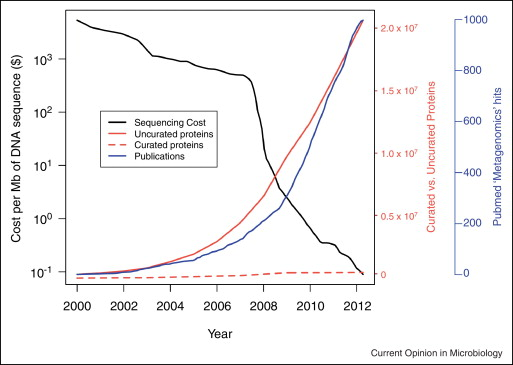
\includegraphics[width=120mm]{conc_figures/seq_vs_curated.jpg}
\caption[Plot of sequencing cost, curated proteins and metagenomic publications from \citet{Temperton2012}]{Plot comparing sequencing cost, uncurated protein data, curated protein data and metagenomics publications from 2000 to 2012 from \citet{Temperton2012}.
Sequencing costs were retrieved from 
\url{http://www.genome.gov./sequencingcosts/}.
Uncurated proteins were the total number of sequences in the UniProt TrEMBL database.
Curated proteins were the total number of manually annotated entries in the SwissProt database.
Metagenomic publications were the total number retrieved from PubMed using the search term `metagenomics'.
}
\label{fig:seq_vs_curated}

\end{figure}

This illustrates how both metagenomics and metaproteomics need to be paired with basic laboratory studies for meaningful biological inferences to continue to be made.
Conversely, it also means a great deal of metagenomics sequences and metaproteomic mass spectra data remains to be taxonomically or functionally assigned.

The specific hypotheses built on environmental data can be used to guide laboratory research studies, such as were detailed above in \emph{Possible future work on Organic Lake}, thus feeding back into supporting a systems-level understanding of microbial communities.
Future `-omic' studies need to now encompass longer time scales and employ focussed analysis of populations and individuals to build on known sequence databases and our biological knowledge base.
Combining `-omics' tools with laboratory work on isolates and with complementary techniques for targeting specific populations, community functions and biogeochemical processes is necessary for a deeper understanding of ecosystems.

\subsection{Metagenomes and metaproteomes are time capsules}
%Although not all of the `-omics' data collected can be assigned to species or function at present, they are still an invaluable resource for the future.
The \textsc{DNA} sequence and mass spectra data that has been produced from these studies form a lasting record of the state of the microbial communities at the point in time that they were collected.
They thus acts as a resource against which other datasets can be compared to gain an understanding of differences between ecosystems and as a bench mark to gauge changes overtime.
These data can also be mined to recover features of interest.
For example genes for enzymes with desired activities or bioactive compounds can be recovered from the sequence information.
As sequence databases grow and more of the microbial world is characterised, this archive of molecular data can be re-analysed to learn even more about the lake ecosystems.

%cite your future work section and other people's commentaries.
%Cite \cite{Warneke2007}
%\figref{fig:prok_diversity} illustrates how much additional bacterial and archaeal taxonomic diversity has been revealed by environmental sequencing and also suggests how much more of their genomic diversity is still undescribed. 
%\begin{figure}[H]
\centering
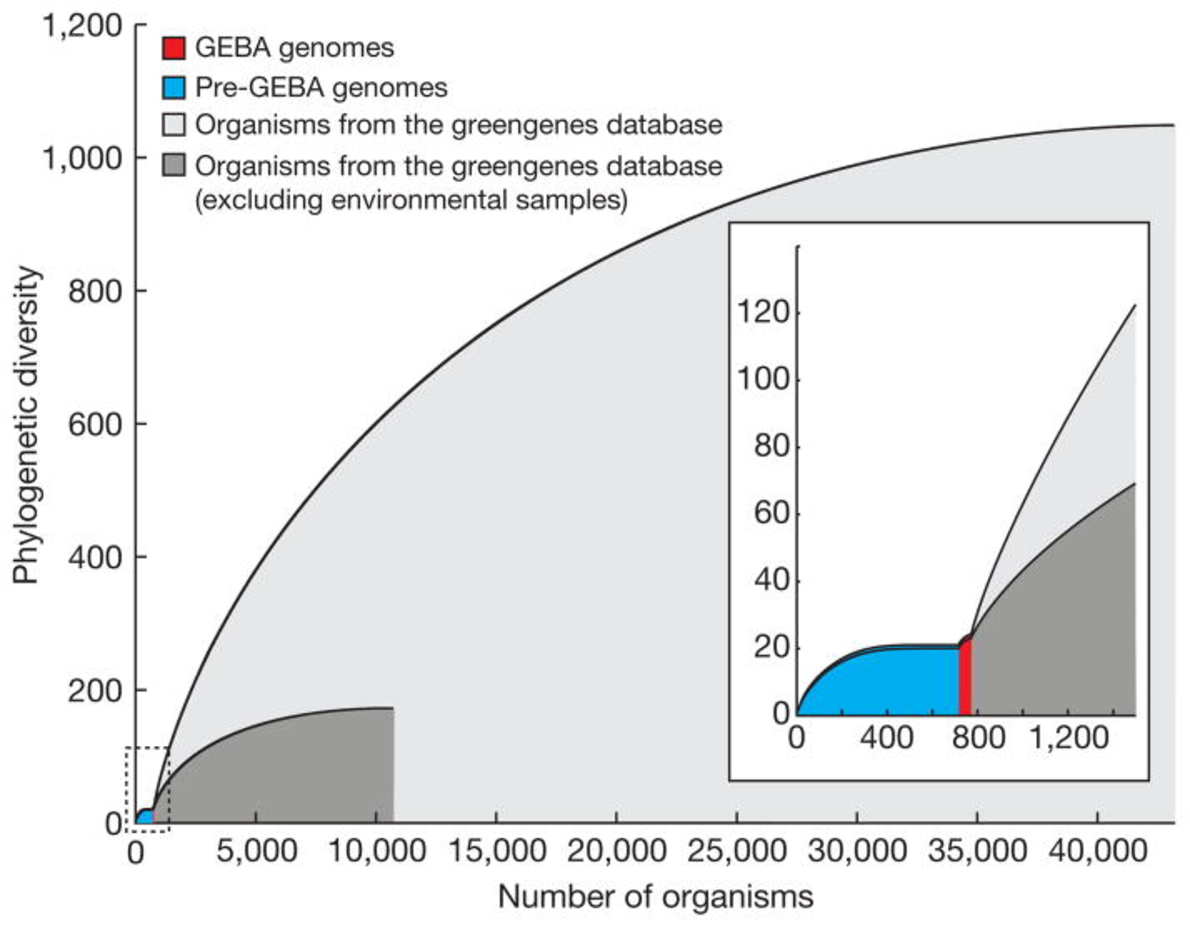
\includegraphics[width=100mm]{conc_figures/prok_diversity.pdf}
\caption[Plot of the diversity of \emph{Bacteria} and \emph{Archaea} from \citet{Wu2009}]{ Plot of the diversity of \emph{Bacteria} and \emph{Archaea} from \citet{Wu2009}. 
The diversity as shown by sequencing of 16S \acp{SSU} genes from the environment, from known organisms and from genomes is compared.
The inset shows the diversity encompassed from sequenced genomes before and after the Genomic Encyclopedia of \emph{Bacteria} and \emph{Archaea} (GEBA) sequencing project, which targets genomes for sequencing based on phylogenetic diverisity \cite{Wu2009}.
}
\label{fig:prok_diversity}

\end{figure}


\section{Concluding remarks}
This thesis has demonstrated how metagenomics and metaproteomics can be used to as tool for characterising Antarctic lake ecosystems.
These datasets represent detailed snap shots of the Ace Lake and Organic Lake microbial communities from which totally new insights into micrbial diversity and functions were gained.
It is also apparent that a complete picture of the lake communities is only beginning to be formed.
As sequence databases and our understanding of the microbial world grows, undoubtedly, more can be interpreted from just these datasets.
In light of the immense potential of sequencing technologies and what has been learnt from the first decades of `-omics' research, future studies can be better equipped to unravel how lakes change over time and build better predictive models of ecosystem function.  
The studies presented here provide a foundation for building an ecosystems level understanding of these exceptional environments.
